\documentclass[12pt,a4paper]
{article}
\usepackage{hyperref}
\usepackage{fancyhdr}
\usepackage{fancybox}
\usepackage{times}
\usepackage{cite}
\usepackage{graphicx}
\usepackage[left=1in,right=0.7in,top=1in,bottom=1in]{geometry}
\usepackage{hyperref}
\usepackage{amsfonts}
\usepackage{epsfig}
\usepackage{subfigure}
\usepackage{amssymb}
\usepackage{times}
\usepackage{graphicx}
\usepackage{setspace}
%\usepackage[left=1.25in,right=1in,top=1in,bottom=1in]{geometry}
%\usepackage{tocloft}
\usepackage{pdfpages}
\usepackage{caption}
\usepackage{chngcntr}
\counterwithin{figure}{section}
\counterwithin{table}{section}
\renewcommand\refname{BIBLIOGRAPHY}
\usepackage[titletoc]{appendix}
\renewcommand{\appendixname}{Annexure}
\usepackage{amsmath}
\numberwithin{table}{section}
%\graphicspath{ {figures/} }
%\usepackage{natbib}
%\begin{document}

\begin{document}
%---------------------------------------Cover Page-------------------------------------------------------
\newpage
\pagestyle{empty}
 %\thispagestyle{empty}
	\pagenumbering{gobble}
	\thisfancyput(-0.0in,-9.5in){%
	%\thisfancypage{%
%\setlength{\fboxrule}{1pt}\doublebox}{} 
\setlength{\unitlength}{1in}\framebox(6.7,10)}

	
	
\begin{center}
	  \begin{figure}[h]
			\centering
			
\includegraphics[width=2 cm , height= 2 cm]{Sppu.jpg}
		\end{figure}
	\end{center}	
	\begin{center}
      \textbf{SAVITRIBAI PHULE PUNE UNIVERSITY , PUNE}  
      
\hspace{0.3 in}

      \textbf{A PROJECT REPORT}
      
\hspace{0.1 in}
       ON
			\end{center}
			
	\begin{center}
		\large\bf{\color{red}\textbf{\Large \lq \lq  LiFi: High Speed Data communication with Security \ \rq \rq}}
	\end{center}
     \vspace{0.1 in}
	
		\begin{center}
	    SUBMITTED TOWARDS THE \\
PARTIAL FULFILMENT OF THE REQUIREMENTS OF
	     
	\end{center}
	
	\begin{center}
	   \textbf{BACHELOR OF ENGINEERING
	   \\ (Computer Engineering)}
	\end{center}
	
	
	\begin{table}[htbp]
\begin{center}
\begin{tabular}{l c c l}
\large\bf{\color{black}Name} & & & \large\bf{\color{black}Exam Seat No.}\\[0.3cm]
\large{\color{black}Nadeem Patil } & & & \large{\color{black}(B120514278)} \\
\large{\color{black}Hemant Badhe } & & & \large{\color{black}(B120514208)}\\
\large{\color{black}Abhijit Jirole } & & & \large{\color{black}(B120514246)}\\ 
\large{\color{black}Pramodini Akhade } & & & \large{\color{black}(B120514203)}\\
\end{tabular}
\end{center}
\end{table}
	\begin{center}
	  \textbf{UNDER THE GUIDANCE OF}\\
	  
	\end{center}
		\begin{center}Prof. Anuja Bharate
	  \begin{figure}[h]
			\centering
			
\includegraphics[width=2.5 cm]{logo.JPG}
		\end{figure}
	\end{center}
		\begin{center}
	  \textbf{DEPARTMENT OF COMPUTER ENGINEERING}\\
	 \textbf{ JSPM's\\
	  IMPERIAL COLLEGE OF ENGINEERING AND RESEARCH,\\
	  WAGHOLI, PUNE 412 207\\2017-18}
	  
	\end{center}
%\end{document}

%------------------Front Page end-----------------



\newpage
\pagestyle{empty}
 %\thispagestyle{empty}
	\pagenumbering{gobble}
	\thisfancyput(-0.0in,-10.0in){%
	%\thisfancypage{%
%\setlength{\fboxrule}{1pt}\doublebox}{} 
\setlength{\unitlength}{1in}\framebox(6.7,10.6)}

\begin{center}

\includegraphics[width=2cm]{logo.JPG}
\end{center}
\begin{center}
{\bf JSPM's\\
IMPERIAL COLLEGE OF ENGINEERING AND RESEARCH,\\
	   DEPARTMENT OF COMPUTER ENGINEERING\\}
%\vspace{0.1in}
\end{center}
\vspace{0.2in}
\begin{center}
\textbf{\underline{{\LARGE {\color{blue}C E R T I F I C A T E}}}}
\vspace{0.1in}
\end{center}
		\noindent
  				\setlength{\baselineskip}{1.2\baselineskip}
	\begin{center}
This is to certify that the Project entitled\\
		\textbf{\large LiFi: High Speed Data communication with Security}\\
\singlespace
Submitted by \\
	\begin{table}[htbp]
\begin{center}
\begin{tabular}{l c c l}
\large\bf{Name} & & & \large\bf{Exam Seat No.}\\[0.3cm]
\large{Nadeem Patil } & & & \large{(B120514278)} \\
\large{Hemant Badhe } & & & \large{(B120514208)}\\
\large{Abhijit Jirole } & & & \large{(B120514246)}\\
\large{Pramodini Akhade } & & & \large{(B120514203)}\\
\end{tabular}
\end{center}
\end{table}
	\end{center}
%\onehalfspace
\begin{quote}
is a bonafide work carried out under the supervision of \textbf{Prof. Anuja Bharate} and it is
submitted towards the partial fulfilment of the requirement of Savitribai Phule Pune\linebreak
University, for the award of the degree of  Bachelor of Engineering .\end{quote}		
\vspace{0.9 cm}
\begin{minipage}[t]{7cm}
\flushleft
\hspace{0.3in} Prof. Prof. Anuja Bharate\\
\hspace{0.55in}(Internal Guide)\\
\hspace{0.30in}(Dept. of Computer Engg.)
\end{minipage}
\hspace{0.5 in}
\begin{minipage}[t]{7cm}
\flushright
\vspace{0.1 in}
 Prof.\hspace*{0.95 in} \\
(External Examiner)
\end{minipage}
\vspace{0.7 in}





\begin{minipage}[t]{7cm}
\flushleft
\hspace{0.1in}Prof. Shital Thokal\\
\hspace{0.35in}(Project Coordinator) 
\hspace{0.9 in}(Dept. of Computer Engg.   )
\end{minipage}
\hspace{0.5 in}
\begin{minipage}[t]{7cm}
\flushright
\hspace{0.65in}Dr. Satish R. Todmal\\
\hspace{0.65in}(Head Of Department)\\
\hspace{0.9 in}(Dept. of Computer Engg.   )
\\
\end{minipage}
\\
 
\newline
\newline
\\
\hspace{0.5in}
Place: Pune \hspace{3.5in} 

\hspace{0.5 in} Date: 

	

%--------------------Certificate ends-------------------





%--------------------------------------------Abstract------------------------------------------------
		\newpage					%start a new page
		 \pagestyle{plain}
%\pagenumbering{roman}
    %\pagenumbering{roman}
		\begin{center}				%centre align the text
			
				\section*{Abstract}
				\addcontentsline{toc}{section}{Abstract}
				\vspace{.15 in}       %leave space of 0.5 inches vertically
			
		\end{center}

		\begin{normalsize}
				\begin{quote}
				{\setlength{\baselineskip}{1.5\baselineskip}%set line spacing as 1.5
				
\hspace{0.7 in}{Data communication or transmission has become the most demanding need for the most of the computer users. Security is another more important concern when it comes to establishing communication between systems through the network. LiFi technology is focused on fulfilling  these demands.LiFi basically uses Visible Light Communication(VLC) to establish connection and transmit data. The transmission rate of visible light is faster than all other available today transmission medias such s WiFi, ethernet, infrared etc. Visible Light Communication has many features such as High speed, no radiation, easy to use, easy installation and management etc. However exiting  LiFi misses out some things such as two way communication, security. So in order to achieve the high speed of LiFi technology and provide transmission security, the proposed system provides the necessary information. }\\



}


				\end{quote}	
		\end{normalsize}
%--------------------------------- Abstract ends



%------------------ack----------------------
\newpage					%start a new page
%\pagestyle{plain}
%\pagenumbering{roman}
\pagestyle{empty}
 %\thispagestyle{empty}
	\pagenumbering{gobble}
							
		\newpage					%start a new page
\pagestyle{plain}
\pagenumbering{roman}
		\begin{center}				%centre align the text
			
				\section*{Acknowledgement}
				 \addcontentsline{toc}{section}{Acknowledgement}
				\vspace{.15 in}       %leave space of 0.5 inches vertically
			
		\end{center}

		\begin{normalsize}
{

				{\setlength{\baselineskip}{1.5\baselineskip}
				It gives us a great pleasure in presenting this Preliminary Project report on "\textbf{LiFi: High Speed Data communication with Security. }" and to express our deep regards towards those who have offered their valuable time and guidance in our hour of need.
				
	\vspace*{.15in}	
	
We would like to express our sincere and whole hearted thanks to our  guide \textbf{Prof. Anuja Bharate} for contributing valuable time, knowledge, experience and providing valuable guidance in making this work a success.


\vspace*{.15in}	

	

We would also like to express our thanks to Project Coordinator \textbf{Prof. Shital Thokal} who
motivated us in successfully completing the Project work.


\vspace*{.15in}	

We would also like to express our thanks to Head of department \textbf{Prof. S. R. Todmal} who
motivated us in successfully completing the Project work.

\vspace*{.15in}	

We are also glad to express our gratitude and thanks to our Principal \textbf{Dr. Dilip D. Shah} for his constant inspiration and encouragement.

\vspace*{.15in}	

Finally, we would like to express once again our gratitude and thanks to all those who are involved directly and indirectly in achieving our project a success.


%\par}

	
}
				\vspace{0.9 in}
				
	\hspace{5 in}			Nadeem Patil
	
	\hspace{5 in}			Hemant Badhe
	
	\hspace{5 in}			Abhijit Jirole
	
	\hspace{5 in}			Pramodini Akhade
	
	
	\hspace{4.5 in}         (Dept. of Computer Engg.)
	
	
			
					
				

%				\end{quote}
			}
		\end{normalsize}

%-----------------------------------Acknowledgement ends-------------------------------------------------


\newpage
\pagestyle{plain}
%\pagenumbering{roman}


				

%--------------------------------- Table of Contents-----------------------------
%\begin{document}
\newpage
\pagestyle{fancy}
						
							
				\begin{normalsize}
				\pagestyle{plain}
					%\pagenumbering{roman}
					%{\setlength{\baselineskip}{1.5\baselineskip}
              				
					\tableofcontents
			      \addcontentsline{toc}{section}{Table of Contents}
			         
			         \newpage
			         \pagestyle{plain}
					%	\pagenumbering{roman}
			         {\setlength{\baselineskip}{1.5\baselineskip}
                      	         
			         \listoffigures
			         \addcontentsline{toc}{section}{List of Figures}
			         }
			         

			         
 \newpage
 {\setlength{\baselineskip}{1.5\baselineskip}
\listoftables
\addcontentsline{toc}{section}{List of Tables}
}			   
 \end{normalsize}
			         

			         
			         
%-------------------------Synopsis----------
%\begin{document}
\newpage
\pagestyle{fancy}
\pagenumbering{arabic}
\fancyhead[RO]{}				% Right over part of header
\fancyhead[LO]{}				% Left over part of header
\renewcommand{\footrulewidth}{0.5pt}	     				% command to change footer ruler width
\fancyfoot[RO]{\textit{JSPM's ICOER, Wagholi, Pune}}								% Right over part of footer
\fancyfoot[LO]{\textit{Department of Computer Engineering}}									% Left over part of footer

% \pagenumbering{arabic}

\newpage

\begin{minipage}{15cm}


\vspace{4 in}
 \begin{center} 
\begin{Huge}
CHAPTER 1

\vspace{0.5 in}

SYNOPSIS
\end{Huge}

\end{center}
\end{minipage}
\newpage
\begin{center}
\section{SYNOPSIS}
\end{center}
 {\setlength{\baselineskip}{1.0\baselineskip} 		
  \vspace{0.1in}	
 
 


\vspace{0.1 in}
\subsection{Project Title}
\vspace{0.1 in}
High Speed Data Communication using LiFi providing Security

\subsection{Project Option }
\vspace{0.1 in}
 Internal project

\subsection{Internal Guide}
\vspace{0.1 in}
Prof. Anuja Bharate


\subsection{Sponsorship and External Guide} 
\vspace{0.1 in}
N/A

\subsection{Problem Statement}
\label{sec:problem}
    \hspace{0.7 in}   Transmission of data between computers is expected to be fast, reliable and secure. The technology used should provide these features. While the data is being transmitted, there should not be any case where data is tampered, stolen or modified by any unauthorised user. The process of data transfer should be fluent and without any additional efforts for the user. Users can be using LiFi in any environmental conditions so the system should withstand any kind of environmental condition with security concern in mind, the data transmission process should have encryption and decryption technology so that users can rely on the system.
\\
\newpage
\subsection{Abstract}

\hspace{0.7 in}\textit{Data communication or transmission has become the most demanding need for the most of the computer users. Security is another more important concern when it comes to establishing communication between systems through the network. LiFi technology is focused on fulfilling  these demands.LiFi basically uses Visible Light Communication(VLC) to establish connection and transmit data. The transmission rate of visible light is faster than all other available today transmission medias such s WiFi, ethernet, infrared etc. Visible Light Communication has many features such as High speed, no radiation, easy to use, easy installation and management etc. However exiting  LiFi misses out some things such as two way communication, security. So in order to achieve the high speed of LiFi technology and provide transmission security, the proposed system provides the necessary information.}  }\\
\\
\subsection{Goals and Objectives}
The proposed system uses Arduino Uno R3-328 and MSP 430 G2 micro controllers. These micro controllers are capable of connecting to personal computers and can be programmed through programming languages.
	The primary goal of the system  is to provide high data transmission rate and should also provide the data security. The data transmission is basically operated by the ON and OFF of the LED and the light received by photo diode. The existing systems are capable of providing the data transmission and security but with the increased data traffic, the speed expectations also increase. LiFi has the ability to fulfil this expectation.
	In a nutshell, LiFi overtakes the existing data transmission techniques in terms of speed and also  provides the transmission security.



\subsection{Relevant mathematics associated with the Project}
\label{sec:math}

{\large { \textbf{Mathematical Model:}}
\\

\hspace{0.7 in}\textit{Let the system be S,

System Description:

S = \{I, O, F, S \}
	\newline Where,
	\newline I= Input from the user in text format or input as a file
	\newline O= Given text or a file at receiver side
	\newline F= Failure condition
	\newline S= Success condition	}
%%%%%%%%%%%%%%%%%%%%%%%%%%%%%%%%%%%%%%%%%%%%%%%%%%
\newpage

\subsection{Names of Conferences / Journals where papers can be published}

\begin{itemize}
\item  	IJCA//Journal 1
\item   Central Universities or SPPU Conferences
\item   IEEE/ACM Conference/Journal 2
\end{itemize}

\subsection{Review of Journal Papers supporting Project idea}
{\small
References: 
\newline \textbf{ 1) "High sensitivity universal LiFi receiver for enhanced data communication"}\\
\textbf{Authors:} Zashi P. Chaudhari, Satish R. Devane\\
\textbf{Description: }In todays world communication between the devices is much common. Radio wave spectrum is very small part of spectrum available for communication but with increase in advanced technology and number of users the network becomes overloaded which results in failure to provide high data rate. Visible light acts as rival to the present wireless radio frequency communication by larger bandwidth and high data rate.\\
\textbf{DOI: }10.1109/GET.2016.7916619\\
\textbf{Year: }2016\\
\newline \textbf{ 2) "LiFi – The path to a New Way of Communication"}\\
\textbf{Authors:} Monica Leba, Simona Riurean, Andreea Lonica\\
\textbf{Description: }Important research efforts have been directed over the past ten years, towards exploring alternative parts of thee electromagnetic spectrum that could potentially offload a large portion of the network traffic from the overcrowded radio frequency(RF) domain. This paper summarizes most of the research , developments and application achieved so farand looks at the different aspects of the strengths and weaknesses, implementations, challenges, VLC IEEE standard and modulation technique of the VLC and specific LiFi's new coined optical wireless communication technology.\\
\textbf{DOI: }10.23919/CISTI.2017.7975997\\
\textbf{Year: }2017\\
\newline \textbf{3)  "Integrated LiFi (Light Fidelity) for smart communication through illumination"}\\
\textbf{Authors:}R. Mahendran\\
\textbf{Description: }The intensity of the LEDs is varied by  alternating the current passed through them at very high speeds. However, the human eye cannot recognize this change and the LEDs appear to have a constant intensity. This ON-OFF activity of LED lights facilitate data transmission using binary codes i.e, when the LED is ON, logical1'1' is transmitted and when the LED OFF, logical '0' is transmitted.\\ 
\textbf{DOI: }10.1109/ICACCCT.2016.7831599\\
\textbf{Year: }2016\\
\newline \textbf{4)  "LiFi: Conceptions, misconceptions and opportunities"}\\
\textbf{Authors: }Harald Hass\\
\textbf{Description: }In this talk we will first explain what Light Fidelity(LiFi) is and highlight the key differences to visible light communication(VLC). We will discuss misconception and illustrate the potential impact this technology can have across a number of existing and emerging industries.\\
\textbf{DOI: }10.1109/IPCon.2016.7834279\\
\textbf{Year: }2016\\
\newline \textbf{5)  "Future internet and Internet of things"}\\
\textbf{Authors: }Pradeep Kumar\\
\textbf{Description: }The future Internet will be capable of connecting and communicating with almost all physical and virtual objects around us to the existing Internet. The Internet of Things is a vision that entails connectivity among different physical and virtual objects in order to understand how the life would change when things, homes and cities become smart.\\
\textbf{DOI: }10.1109/ICIEECT.2017.7916594\\
\textbf{Year: }2017\\
\newline \textbf{6) "Prototyping and measurements for a LiFi system"}\\
\textbf{Authors: }Kun Chen Hu\\
\textbf{Description: }The prototype is based on two Spartan 6 FPGAs and uses a Light Emitting Diode (LED) to transport the information through amplitude changes of the light. The receiver uses a low dark current PIN photodiode. We describe the system design, the receiver algorithms and the measurement set-up. We present some measurements where in a Line of Sight (LOS) channel the received pulses are shown to match the transmitted ones.\\
\textbf{DOI: }10.1109/SAM.2016.7569701\\
\textbf{Year: }2016\\
\newline \textbf{7) "Digital data transmission via visible light communication(VLC): Application vehicle to vehicle communication"}\\
\textbf{Authors: }Dahmani Mohammed\\
\textbf{Description: }Visible Light Communication(VLC) may improve driver's safety by allowing the vehicles to communicate easily with each other (V2V communication). The first prototype of an unidirectional VLC communication was developed at the laboratory of signals and images (LSI) of USTO-MB. The experimental results are more than satisfactory.\\
\textbf{DOI: }10.1109./CEIT.2016.7929059\\
\textbf{Year: }2016\\
\newline \textbf{8) "Impact of VLC on Light Immission Quality of White LEDs"}\\
\textbf{Authors: }Wasiu O. Popoola\\
\textbf{Description: }This paper reports the effect of data modulation on the emitted light quality of phosphor converted white LEDs. The results showed that provided the expected average current driving the LEDs remains unchanged then the emitted light quality will stay the same. For a dc-balanced modulating signal, with a nonvarying average value, any fluctuations in the instantaneous driving current due to data modulation do not have any significant impact on the measured light quality metrics. \\
\textbf{DOI: }10.1109/JLT.2016.2542110\\
\textbf{Year: }2016\\
\newline \textbf{9) "On visible light communication and quality of light emitted from illumination LEDs"}\\
\textbf{Authors: }Wasiu O.Popoola\\
\textbf{Description: }We present the effect of LiFi, with on-off keying modulation technique, on the quality of light emitted from LEDs. Findings show that to preserve the LED light quality, the LiFi data signal should be such that the LED average drive current remains unchanged.\\
\textbf{DOI: }10.1109/PHOSST.2016.7548765\\
\textbf{Year: }2016\\
  
  
  \newpage
  
  \subsection{Plan of Project Execution}
\textbf{PROJECT ESTIMATES} \\ 
Waterfall approach we use an SDLC Model widely in Software Engineering to ensure success of the project. In "The Waterfall" approach, the whole process of software development is divided into separate phases. In this Waterfall model, typically, the outcome of one phase acts as the input for the next phase sequentially. The following illustration is a representation of the different phases of the Waterfall Model.

 \begin{figure}[h]
\centering
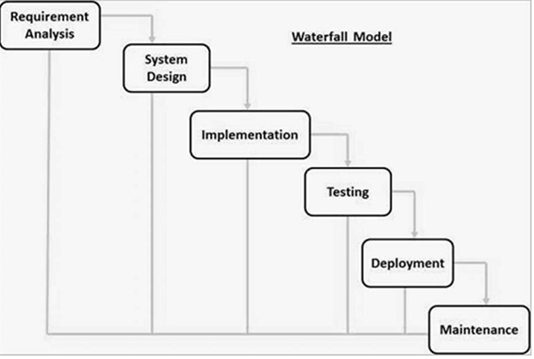
\includegraphics[width=15cm , height=10 cm]{img.PNG}
%\includegraphics[width=0.9\linewidth]{snap}
\caption{Project Plan} 
\label{fig: Project Plan}
\end{figure}

  
  
  
  
  
  
%------------------------------------technical keywords-----------
\newpage
\begin{minipage}{15 cm}


\begin{center} 
\begin{Huge}
\vspace{4 in}
CHAPTER 2

\vspace{0.2 in}
TECHNICAL KEYWORDS

\end{Huge}

\end{center}
\end{minipage}

\newpage
\begin{center}
\section{TECHNICAL KEYWORDS}
\end{center}
 {\setlength{\baselineskip}{1.0\baselineskip} 		
  \vspace{0.1in}					



 \vspace{0.5 in}
\subsection{AREA OF PROJECT}
Networking and Communication 
	\begin{flushleft}
\subsection{TECHNICAL KEYWORDS}	

	
			\begin{itemize}
			
		
			
				\item \textbf{1.C  Computer Systems Organization} \\
				Computer organization helps optimize performance based products. For example, software engineers need to know the processing power of processors. They may need to optimize software in order to gain the most performance for the lowest price. This can require quite detailed analysis of the computer's organization. For example, in a SD card, the designers might need to arrange the card so that the most data can be processed in the fastest possible way.


				\textbf{ i.Arduino controller} \\
				Arduino is an open-source electronics platform based on easy-to-use hardware and software. Arduino boards are able to read inputs - light on a sensor, a finger on a button, or a Twitter message - and turn it into an output - activating a motor, turning on an LED, publishing something online. You can tell your board what to do by sending a set of instructions to the microcontroller on the board. To do so you use the Arduino programming language (based on Wiring), and the Arduino Software (IDE), based on Processing.

Over the years Arduino has been the brain of thousands of projects, from everyday objects to complex scientific instruments. A worldwide community of makers - students, hobbyists, artists, programmers, and professionals - has gathered around this open-source platform, their contributions have added up to an incredible amount of accessible knowledge that can be of great help to novices and experts alike.
			   \item \textbf{A. Wireless Communication} \\
			    Wireless communication, or sometimes simply wireless, is the transfer of information or power between two or more points that are not connected by an electrical conductor. Wireless operations permit services, such as long-range communications, that are impossible or impractical to implement with the use of wires. Wireless data communications allows wireless networking between desktop computers, laptops, tablet computers, cell phones and other related devices. The various available technologies differ in local availability, coverage range and performance.
		
				
		\end{itemize}



	\end{flushleft}
%--------------keywords ends here






%------------------------introduction---------------
\newpage


\begin{minipage}{15cm}


\vspace{4 in}
 \begin{center} 
\begin{Huge}
CHAPTER 3

\vspace{0.5 in}

INTRODUCTION
\end{Huge}

\end{center}
\end{minipage}
\newpage

\begin{center}
\section{INTRODUCTION}
\end{center}
 {\setlength{\baselineskip}{1.0\baselineskip} 		
  \vspace{0.1in}			
  
  \vspace{15 pt}
 }
 
\subsection{PROJECT IDEA}
\vspace{0.1 in}
\begin{itemize}	
Data communication or the transmission among various systems is the most commonly used feature of the computer systems. There are various data transmission methods such as wired communication, wireless communication. Ethernet, WiFi, Bluetooth are the widely used data transmission protocols. With the increasing number of computer users, the data storage capacities and data requirements are increasing tremendously. The existing systems are facing various issues such as traffic overloading , data bottleneck,  bandwidth overloading etc. To overcome these issues, we require even the higher bandwidth than existing systems. LiFi has the capability to fulfil this demand so, bringing the LiFi technology in use can solve many issues. Additionally, security needs to be maintained for data integrity and reliability. The basic idea of the project is to reduce bandwidth overloading, network traffic, communication restrictions in sensitive areas etc and provide secure, reliable and easy to use system for users.
\end{itemize}
\vspace{0.4 in}

\subsection{MOTIVATION OF THE PROJECT}
\vspace{0.1 in} 
\begin{itemize}
\item	Traditional data transmission techniques are capable of handling most of the data traffic all over the internet, however it is not sufficient for managing all the traffic. What motivates to this paper is the speed limitation, bandwidth limitation, transmission restriction of the traditional transmission protocols. 
\item Security is becoming an important concern among the computer users. To come up with satisfying this concern, our idea here suggest and puts forward the methods of providing the security have motivated this project to provide additional security to the transmission technology.
\item The paper suggest various method of data transmission. The transmission devices are portable, the communication can be achieved between desktop computers, mobile computing devices or a desktop and a mobile computing device.
\item Also, the motivations behind this project are the unavailability of existing communication techniques in some areas such as underwater communication, communication on high lattitude areas(ex. communication from one station on a mountain to other sttation on another mountain).
\end{itemize}



\newpage
\subsection{LITERATURE SURVEY}

\begin{table}[htbp]
\begin{center}
\begin{tabular}{|p{25pt}|p{100pt}|p{85pt}|p{180pt}|}
\hline
\textbf{Sr.} \par \textbf{No. }\par & 
\textbf{Paper Title} \par & 
\textbf{Author} & 
\textbf{Analysis} \\
\hline
1& 
High sensitivity universal LiFi receiver for enhanced data communication & 
 Zashi P. Chaudhari, Satish R. Devane & 
In todays world communication between the devices is much common. Radio wave spectrum is very small part of spectrum available for communication but with increase in advanced technology and number of users the network becomes overloaded which results in failure to provide high data rate. Visible light acts as rival to the present wireless radio frequency communication by larger bandwidth and high data rate. \\
\hline
2& 
LiFi The path to a New Way of Communication  & 
Monica Leba, Simona Riurean, Andreea Lonica\textit{\textdagger } & 
Important research efforts have been directed over the past ten years, to-
wards exploring alternative parts of thee electromagnetic spectrum that could potentially
offload a large portion of the network traffic from the overcrowded radio frequency(RF) do-
main. This paper summarizes most of the research , developments and application achieved
so far and looks at the different aspects of the strengths and weaknesses, implementations,
challenges, VLC IEEE standard and modulation technique of the VLC and specific LiFi's
new coined optical wireless communication technology. \\
\hline
3& 
Integrated LiFi (Light Fidelity) for smart communication through illumi-
nation  & 
R. Mahendran  & 
The intensity of the LEDs is varied by alternating the current passed through
them at very high speeds. However, the human eye cannot recognize this change and the
LEDs appear to have a constant intensity. This ON-OFF activity of LED lights facilitate
data transmission using binary codes i.e, when the LED is ON, logical1'1' is transmitted
and when the LED OFF, logical '0' is transmitted. \\
\hline



\label{tab1}
\end{tabular}

\end{center}
\end{table}

\begin{table}[htbp]
\begin{center}
\begin{tabular}{|p{25pt}|p{100pt}|p{85pt}|p{180pt}|}
\hline
\textbf{Sr.} \par \textbf{No. }\par & 
\textbf{Paper Title} \par & 
\textbf{Author} & 
\textbf{Analysis} \\
\hline
4&
Prototyping and measurements for a LiFi system &
Kun Chen Hu &
The prototype is based on two Spartan 6 FPGAs and uses a Light Emitting
Diode (LED) to transport the information through amplitude changes of the light.
The receiver uses a low dark current PIN photodiode. We describe the system design, the receiver
algorithms and the measurement set-up. We present some measurements where in a Line
of Sight (LOS) channel the received pulses are shown to match the transmitted ones.
\\
\hline
5&
Digital data transmission via visible light communication(VLC): Applica-
tion vehicle to vehicle communication &
Dahmani Mohammed &
Visible Light Communication(VLC) may improve driver's safety by allowing
the vehicles to communicate easily with each other (V2V communication). The first pro-
totype of an unidirectional VLC communication was developed at the laboratory of signals
and images (LSI) of USTO-MB. The experimental results are more than satisfactory.\\
\hline
6&
On visible light communication and quality of light emitted from illumi-
nation LEDs &
Wasiu O.Popoola &
We present the effect of LiFi, with on-off keying modulation technique, on
the quality of light emitted from LEDs. Findings show that to preserve the LED light
quality, the LiFi data signal should be such that the LED average drive current remains
unchanged.\\
\hline

\label{tab1}
\end{tabular}
\end{center}
\end{table}

\newpage






%---------------intro ends here------------





%-----------------PROBLEM DEFINITION AND SCOPE-----------
\newpage

\begin{minipage}{15cm}


\vspace{4 in}
 \begin{center} 
\begin{Huge}
CHAPTER 4

\vspace{0.5 in}

PROBLEM DEFINITION AND SCOPE
\end{Huge}

\end{center}
\end{minipage}

\newpage
\begin{center}
\section{PROBLEM DEFINITION AND SCOPE}
\end{center}
 {\setlength{\baselineskip}{1.0\baselineskip} 		

  

\hspace{50pt}



\subsection{PROBLEM STATEMENT}

\par \hspace{0.2 in}Data communication or transmission has become the most demanding need for the most of the computer users. Security is another more important concern when it comes to establishing communication between systems through the network. LiFi technology is focused on fulfilling  these demands.LiFi basically uses Visible Light Communication(VLC) to establish connection and transmit data. The transmission rate of visible light is faster than all other available today transmission medias such s WiFi, ethernet, infrared etc. Visible Light Communication has many features such as High speed, no radiation, easy to use, easy installation and management etc. However exiting  LiFi misses out some things such as two way communication, security. So in order to achieve the high speed of LiFi technology and provide transmission security, the proposed system provides the necessary information.

\subsubsection{Goals and Objectives}

 The objectives of this project are:
 \begin{enumerate}
\item Upgrade existing data communication techniques to provide faster, reliable , secure and easy to use communication technology.

\item Provide a system which can withstand in any physical environment. To reach out in the areas where existing communication aren't able to reach.
\item It is also taken in consideration that the provided system matches the safety needs of using an electrical device. The devices are safe to use and shall not harm any human or shell not damage any human resources.

\item The primary goal of this project is to fulfil the speed demands and to provide secure communication techniques which  will replace some of the existing system, but will also be an addition in the techniques without affecting any other communication medium. \\
\end{enumerate}

\subsubsection{Scope of Project}
To ensure the effectiveness of our proposed system, we can some tests. Arduino microcontroller is connected with a 
desktop system. The Arduino IDE is used for programming the microcontroller. We are using Java programming language(Object Oriented).
	The microcontroller is connected with the Light Emitting Diode. This microcntroller is programmed through the desktop system which controls the LED. This LED is the data emission device. We will be using a photo diode as a receiving device which will also be connected to another desktop system  which will act as a receiver device. The tests were passed by the setup and hence further improvements can be made  in the system.  
\subsection{SOFTWARE CONTEXT}
For developing our project , we require IDE's IntelliJ IDEA and Arduino IDE, Java as a programming language(OOP). We are also using various electrical devices such as LEDs, Bread Boards, Jumper Wires etc for implementation.

\subsection{MAJOR CONSTRAINTS}
Major Constraints in these project can be transmitting data from one device to another and also manage the whole system structure.



\subsection{OUTCOME}
\begin{itemize}
The speed of transmission varies with various factors such as light intensity, read-write speed, physical distance, etc. If the device are placed close(<10m), the system can provide least transmission speed of 10MB/s, however improvements are being made and speed in GBs can be achieved soon. The system is cost effective and fulfils the transmission demands.\\
Drawbacks of proposed system:\\
i) Transmission cannot be made when there is any physical  obstacle.\\
ii) Saturation and stabilization of system can take two more years.

\end{itemize}



\subsection{HARDWARE RESOURCES REQUIRED}
1.	RAM :- 4GB or Higher \\
2.	CPU :- 2Ghz or Higher
3.  Processor: Intel Pentium IV or above\\
5.  HDD: 500 GB \\
6.  Keyboard and Mouse: QWERTY  Wired or Wireless \\

\subsection{SOFTWARE RESOURCES REQUIRED}
1.	Operating System:- Windows 7 or above/Linux(All distribution)\\
2.	Platform:- Java, Arduino studio \\
3.	IDE:- IntelliJ IDEA, Arduino IDE and sCode Blocks. \\
4.	Programming Language:- Java, C \\




%--------------------PROBLEM DEFINITION AND SCOPE here-------








%-----------------Project plan-----------
\newpage
\begin{minipage}{15cm}


\vspace{4 in}
 \begin{center} 
\begin{Huge}
CHAPTER 5

\vspace{0.5 in}

PROJECT PLAN
\end{Huge}

\end{center}
\end{minipage}

\newpage
\begin{center}
\section{PROJECT PLAN}
\end{center}
 {\setlength{\baselineskip}{1.0\baselineskip} 		


\subsection{PROJECT ESTIMATES}
\subsubsection{Reconciled Estimates}

\hspace{20 pt}
\textbf{{\small Cost Estimate}} \\
1. IntelliJ IDEA for software development \\
2. IDE – Open Source \\ 
3. Hardware and Software cost – minimum 2 computer with any configuration   (min. cost ₹ 30,000/-)

\vspace{0.1 in}
{\small \textbf{Time Estimates}}\\
9 -10 months
	
\vspace{0.1 in}

\subsubsection{Project Resources}

\vspace{0.1 in}
\hspace{20 pt}
\textbf{People} \\
1.	Internal Guide :- Prof. Anuja Bharate \\
2.	Developers: - Nadeem Patil, Hemant Badhe, Abhijit Jirole, Pramodini Akhade. 

\vspace{0.2 in}
\textbf{Hardware} \\
1.	RAM :- 4GB or Higher \\
2.	CPU :- 2Ghz or Higher 
 
 \vspace{0.2 in}
\textbf{Software} \\
1.	Operating System:- Windows/Linux \\
2.	Platform:- Java  \\
3.	IDE:- IntelliJ Idea ,Arduino IDE  \\
4.	Programming Language:- Java and C.


\newpage


\subsection{RISK MANAGEMENT w.r.t. NP HARD ANALYSIS}
Risk management is the identification, assessment, and prioritization of risks followed by coordinated and economical application of resources to minimize, monitor, and control the probability and/or impact of unfortunate events or to maximize the realization of opportunities. \\ 
Risk management’s objective is to assure uncertainty does not deflect the endeavour from the business goals.  Risks can come from various sources including uncertainty in financial markets, threats from project failures (at any phase in design, development, production, or sustainment life-cycles), legal liabilities, credit risk, accidents, natural causes and disasters, deliberate attack from an adversary, or events of uncertain or unpredictable root-cause.

\subsubsection{Risk Identification}

Our development identified some potential risks to the project. These risks were analyzed and were classified into various categories depending upon the threat they posed to the project. Some of these risks were generic risks while others were product specific risks. A considerable amount of time was spent in analyzing the product specific risks.\\

1.	Have top software and customer managers formally committed to support the project?\\
The software manager and the customer mangers are fully committed to the project.\\

2.	Are end-users enthusiastically committed to the project and the system/product to be built? \\
The end-users have also committed to the project and to the product to be built.\\

3.	Are requirements fully understood by the software engineering team and its customers? \\
Requirements for customer are fully understood by whole team from consistent feedback of customer.\\	


4.	Have customers been involved fully in the definition of requirement?\\
Yes, citizens have been fully consulted and are involved in the process. \\


5.	Do end-users have realistic expectations?\\
End users tend to have some unrealistic expectations, typically, on the various features of the product to be quickly delivered in a constrained manner. \\


6.	Does the software engineering team have the right mix of skills?\\
The team consists of the people with Managerial, Designing as well as developing skill set. \\



7.	Are project requirement stable? \\
Project requirements are stable \\

8.	Is the number of people on the project team adequate to do the job? \\
Number of people to do the job, are adequate, but interns may be necessary as the users grow in size. \\

9.	Do all customer/user constituencies agree on the importance of the project and on the requirements for the system/product to be built? \\
Citizens have consistently agreed on the parameters of the project and its feasibility, and of the requirements for product to be built effectively. \\

\newpage

\subsubsection{Risk Analysis}
The risks for the Project can be analyzed within the constraints of time and quality


\begin{table}[htbp]
\begin{center}
\begin{tabular}{|p{26pt}|p{136pt}|p{70pt}|l|l|l|}
\hline
\raisebox{-1.50ex}[0cm][0cm]{ID}& 
\raisebox{-1.50ex}[0cm][0cm]{Risk Description}& 
\raisebox{-1.50ex}[0cm][0cm]{Probability}& 
& 
Impact& 
 \\
\cline{4-6} 
 & 
 & 
 & 
Schedule& 
Quality& 
Overall \\
\hline
1& 
Hardware Failure& 
High& 
High& 
High& 
High \\
\hline
2& 
Software Failure& 
Medium& 
High& 
Medium& 
Medium \\
\hline
3& 
Input and Output Data & 
Low& 
Low& 
Low& 
Low \\
\hline
\end{tabular}
\caption{Risk Table}
\label{tab1}
\end{center}
\end{table}

%--------------2nd table----------


\begin{table}[htbp]
\begin{center}
\begin{tabular}{|p{71pt}|l|l|}
\hline
Probability& 
Value& 
Description \\
\hline
High& 
Probability of occurrence is& 
\textgreater 75{\%} \\
\hline
Medium& 
Probability of occurrence is& 
26 to 75{\%} \\
\hline
Low& 
Probability of occurrence is& 
\textless 25{\%} \\
\hline
\end{tabular}
\caption{Risk Probability definitions}
\label{tab1}
\end{center}
\end{table}


\subsubsection{Overview of Risk Mitigation, Monitoring, Management}
Following are the details of each risk:-
\begin{table}[htbp]
\begin{center}
\begin{tabular}{|l|p{300pt}|}
\hline
\textbf{Risk ID}& 
1 \\
\hline
\textbf{Risk Description}& 
Hardware failure during Data Transmission, power supply failure, etc.\\
\hline
\textbf{Category}& 
Software failure where Software not launched properly. \\
\hline
\textbf{Source}& 
Many Software problems can take place in an Hardware problem \\
\hline
\textbf{Probability}& 
Medium \\
\hline
\textbf{Impact}& 
High \\
\hline
\textbf{Response}& 
Complete system stops working \\
\hline
\textbf{Strategy}& 
Check the Hardware connections and Restart system. Replace a non working Hardware.
\\
\hline
\textbf{Risk Status}& 
May occur \\
\hline
\end{tabular}
\caption{Risk Impact definitions 1} 
\label{tab1}
\end{center}
\end{table}
%----------------table 2-------------


\begin{table}[htbp]
\begin{center}
\begin{tabular}{|l|p{300pt}|}
\hline
\textbf{Risk ID}& 
2 \\
\hline
\textbf{Risk Description}& 
Software failure, Power supply failure, Hardware not working properly\\
\hline
\textbf{Category}& 
Software didn't detect Hardware device\\
\hline
\textbf{Source}& 
Commodity Hardware \\
\hline
\textbf{Probability}& 
Low \\
\hline
\textbf{Impact}& 
Medium \\
\hline
\textbf{Response}& 
Software will not show connected Hardware devices.
\\
\hline
\textbf{Strategy}& 
Establish connection properly  \\
\hline
\textbf{Risk Status}& 
May occur \\
\hline
\end{tabular}
\caption{Risk Impact definitions 2 }
\label{tab1}
\end{center}
\end{table}

%---------------table 3------------


\begin{table}[htbp]
\begin{center}
\begin{tabular}{|l|p{300pt}|}
\hline
\textbf{Risk ID}& 
3 \\
\hline
\textbf{Risk Description}& 
Data sent from one device is not being received by another \\
\hline
\textbf{Category}& 
Software environment and Hardware connection  \\
\hline
\textbf{Source}& 
General hardware connections \\
\hline
\textbf{Probability}& 
Medium \\
\hline
\textbf{Impact}& 
Medium \\
\hline
\textbf{Response}& 
Sent and/or received data not showing up\\
\hline
\textbf{Strategy}& 
Restart system and check for connection.\\
\hline
\textbf{Risk Status}& 
May occur \\
\hline
\end{tabular}
\caption{Risk Impact definitions 3 }
\label{tab1}
\end{center}
\end{table}

\newpage
 
\subsection{PROJECT SCHEDULE}
\subsubsection{Project task set}
Major task in the project stages are:
\begin{itemize}



\item	Task 1:	Literature survey
\item	Task 2: System analysis
\item	Task 3: Learning required technology
\item	Task 4: Looking for New Methodology 
\item	Task 5: Design and planning
\item	Task 6: New System architecture analysis
\item	Task 7: Implementation
\item	Task 8: System Testing
\item	Task 9: Initial Report
\item	Task 10: Final Report
	\end{itemize}


\subsubsection{Task network}

\begin{center}
	  \begin{figure}[h]
			\centering
			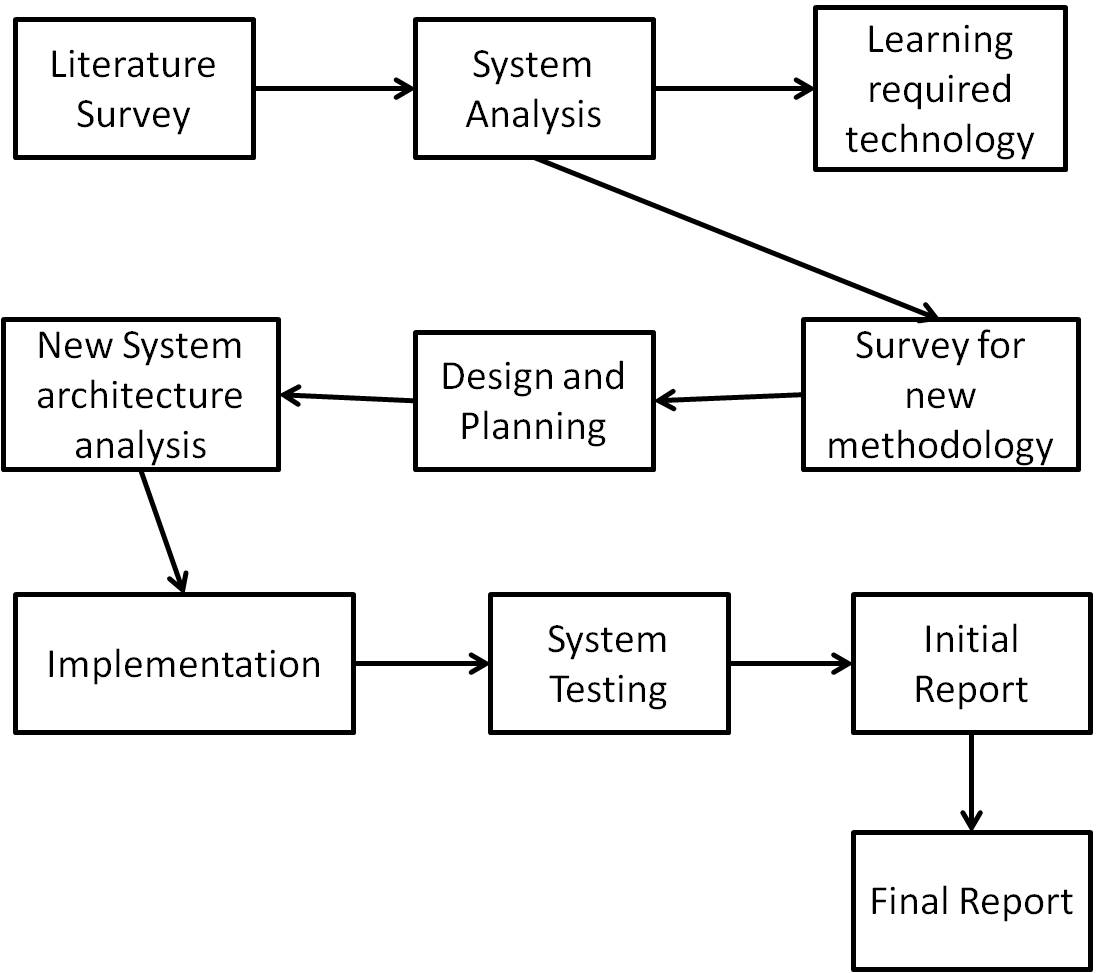
\includegraphics[width=12 cm , height= 6 cm]{TN.jpg}
			\caption{Task network}
		\end{figure}
	\end{center}	
	
	\newpage
	
\subsubsection{Timeline Chart}
\begin{center}
	  \begin{figure}[h]
			\centering
			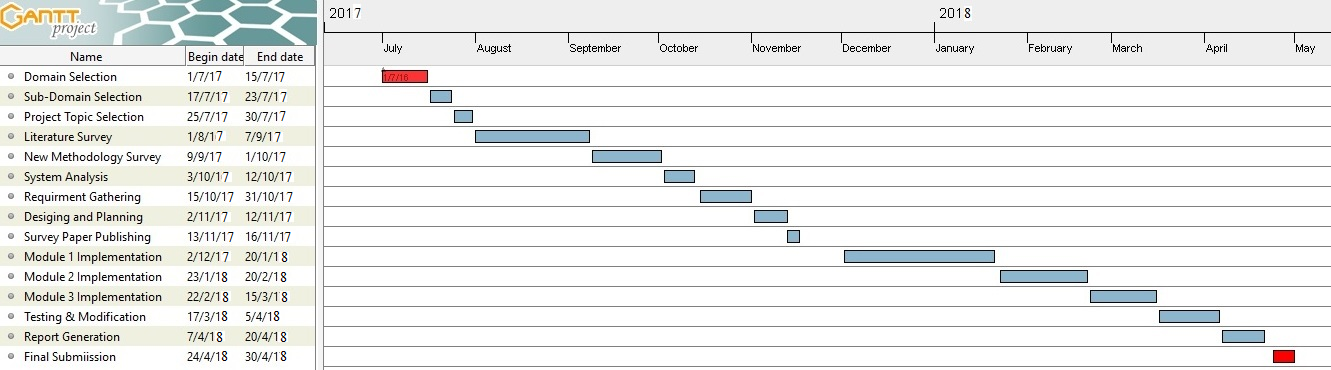
\includegraphics[width=17 cm , height= 8 cm]{TC.png}
			\caption{Timeline Chart}
		\end{figure}
	\end{center}

\vspace{0.4 in}

\subsection{TEAM ORGANIZATION}

Developers and Designers: \\
		\textbf{Design : }	Nadeem Patil, Hemant Badhe, Abhijit Jirole. \\
		\textbf{Backend:}	Hemant Badhe, Abhijit Jirole, Pramodini Akhade. \\
		\textbf{Frontend:}	Nadeem Patil, Abhijit Jirole, Hemant Badhe. \\
		\textbf{Documentation:}	Pranodini Akhade, Abhijit Jirole ,Nadeem Patil . \\
		\textbf{Testing:}	Hemant Badhe, Nadeem Patil, Pramodini Akhade, Abhijit Jirole. \\
\newpage
\subsubsection{Team structure}

	Nadeem Patil	:	Designing, Development, Documentation, . \\
	Hemant Badhe	:	Designing, Development, Testing. \\
	Abhijit Jirole	:	Designing, Development, Testing. \\
	Pramodini Akhade :	Documentation,Designing ,Development.

\subsubsection{Management reporting and communication}

Mechanisms for progress reporting and inter/intra team communication are identified as per assessment sheet and lab time table. 

Intercommunication:	Via Mail or Call


%--------------------project plan ends here-------








%---------SOFTWARE REQUIREMENT SPECIFICATION----------
\newpage
\begin{minipage}{15cm}


\vspace{4 in}
 \begin{center} 
\begin{Huge}
CHAPTER 6

\vspace{0.5 in}
SOFTWARE REQUIREMENT SPECIFICATION
\end{Huge}

\end{center}
\end{minipage}

\newpage
\begin{center}
\section{SOFTWARE REQUIREMENT SPECIFICATION }
\end{center}
 {\setlength{\baselineskip}{1.0\baselineskip} 		
  \vspace{0.1in}


\subsection{INTRODUCTION}

\hspace{10 pt}	Nowadays,the transmission of data is becoming one of the most common factors among the computing devices. Various ways of data transmission have been enhanced such as WiFi, Bluetooth, etc. One of the most concerned issue about data transmission is data transmission security. A method needs to be developed which  will be provide both high speed data transmission as well as data transmission security. LiFi system is one of the emerging technology which is fast and easy to use.\\

\hspace{10 pt}Various methods are available today which provide data transmission feature among various devices. These can be wired or wireless protocols. However these protocols have been some limitations are filled up by LiFi data communication techniques. LiFi is advantages for achieving large data bandwidth which is the demand of the network using crowd.\\

\hspace{10 pt}Some of the network protocols are almost unusable in few situation. For example,WiFi cannot used in establishing connection between two mountains. Another example can be communicating with submarines and the ships, which can also be achieved with the LiFi.
\newpage
\subsubsection{Purpose and Scope of Document}

\hspace{10 pt}
\textbf{Purpose: }	The usage of data communication have been vastly increased from the past decade due to introduction of some high speed internet providing facilities. this introduced facilities played vital role to fulfil user demands. However, with the growth of users and user's data, the bottleneck issue may also produced. The supply or request for data is too much with respect to available bandwidth. LiFi kills this major issue with its high bandwidth. The purpose of introducing this method was to provide high bandwidth and also to providing to necessary data security to each user. It also focuses on reaching out to these areas where existing data transmission method fail to reach. \\
		
\textbf{Scope:}	The main objective is to build data transmitting setup that can provide high speed that can provide high speed data communication among different devices. his should also be available with the security features which does not allow any kind of data insecurity such as data breaching, data leaking, MITM attack, etc.  Establish a secure connection between sender and receiver\\
· Build an interface for the system.\\
· Communicate transmitting and  receiving devices. \\

\subsubsection{Overview of responsibilities of Developer}
\setlength{\baselineskip}{1.5\baselineskip}
The following activities are carried out: \\
{Documentation}:	Pramodini Akhade, Abhijit Jirole, Hemant Badhe \\
{Design:}		Nadeem Patil, Hemant Badhe, Pramodini Akhade \\
{Development:}		Abhijit Jirole, Hemant Badhe, Nadeem Patil\\
{Testing:}		Pramodini Akhade, Nadeem Patil, Abhijit Jirole \\


\subsection{USAGE SCENARIO}
\subsubsection{User profiles}

\textbf{User:}User can select which files to be sent and to which receiver.\\
\textbf{System: }System manages to establish connection between two devices.\\

%\subsubsection{Use-cases}

%\begin{table}[htbp]
%\begin{center}
%\begin{tabular}{|l|l|l|l|l|}
%\hline
%Sr. No.& 
%Use Case& 
%Description& 
%Actors& 
%Assumptions \\
%\hline
%1& 
%System Use Case& 
%Shows the working and cases of the project& 
%user, system.& 
%user, system is software program as well as hardware device . Assume as user. \\
%\hline
%\end{tabular}
%\label{tab1}
%\end{center}
%\end{table}



\subsubsection{Use Case View}
\begin{center}
	  \begin{figure}[h]
			\centering
			\includegraphics[width=18 cm , height= 15 cm]{UseCase.PNG}
			\caption{Use Case Diagram}
		\end{figure}
	\end{center}
	
	\newpage



\subsection{FUNCTIONAL MODEL AND DESCRIPTION}
\subsubsection{Data Flow Diagram}
Data Flow Diagram DFD or data flow diagram is a graphical representation of the flow of data through the information system modelling its process aspects. DFD is often uses as preliminary step to create an overview of the system which can be later elaborated. DFD are also known as bubble chart. DFD is designing tool used in top down approach to system design. \\ This context level DFD is next uploaded to produce Level1 DFD. Level 1 DFD shows how system is divided into sub system each of which deals with one or more to or from man external agent and which together provide all functionality of system as a whole. It also identifies internal data store that must be present in order for the system to do its job and shows the flow of data between various parts of system.
\begin{center}
	  \begin{figure}[h]
			\centering
			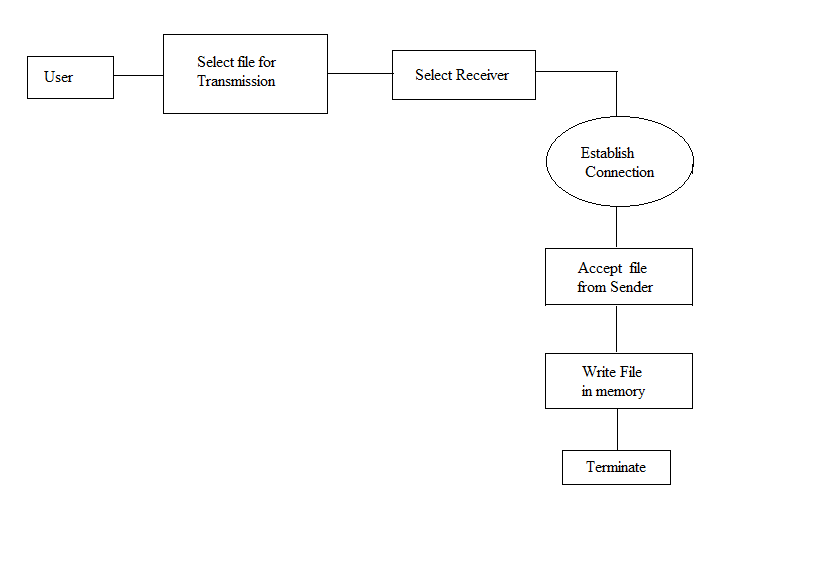
\includegraphics[width=18 cm , height= 12 cm]{DFD.PNG}
			\caption{DFD Level-0}
		\end{figure}
	\end{center}
	
	
\newpage
\subsubsection{Description of functions}
\textbf{user:} user can check notification on app and send message if do further operation.\\
\textbf{system: }it check motion and send signal to an android application .\\

\newpage
\subsubsection{Sequence Diagram}
\begin{center}
	  \begin{figure}[h]
			\centering
			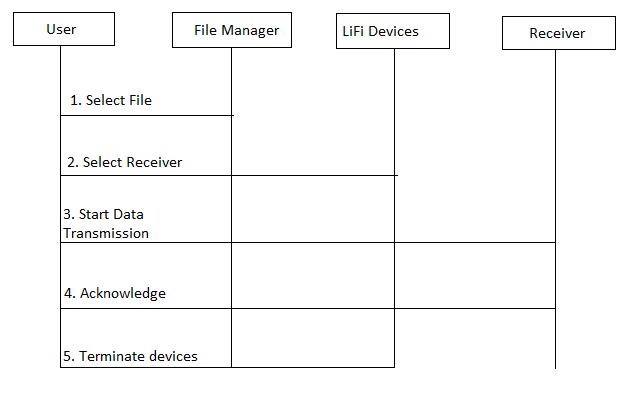
\includegraphics[width=18 cm , height= 12cm]{S.png}
			\caption{Sequence Diagram}
		\end{figure}
	\end{center}
	
\newpage
\subsubsection{{\large Non Functional Requirements:}}
\setlength{\baselineskip}{0.85\baselineskip}
\hspace{10 pt}
\textbf{Interface Requirements:} The interface should be easy to use and intuitive. 
Performance Requirements: The system should give an effective and high performance. \\

\textbf{Software quality attributes:} Availability, Reliability, Reusability, Scalability, Performance, and Usability. The system considers following non-functional requirements to provide better functionalities and usage of system.\\

\textbf{Usability:} The system is designed keeping in mind the usability issues considering the end-users who are developers/programmers. Effort required in learning, operating, preparing input, and interpreting output are to be minimized. It provides detailed help which would lead to better and faster learning. Navigation of system is easy. \\

\textbf{Agility:} Improves with users able to rapidly and inexpensively re-provision technological infrastructure resources. The cost of overall computing is unchanged, however, and the providers will merely absorb upfront costs and spread costs over a longer period. \\

\textbf{Consistency:} Uniformity in layout, screens, colours scheme, via dynamic ("on-demand") provisioning of resources on basis near real-time, without users having to engineer for peak loads.\\ 

\textbf{Performance:} Performance depends on the user’s familiarity with the usage of the system. \\


\textbf{Extendibility:} Templates can be imported from different applications, adding more features in work flow.\\
 
\textbf{Reusability:} The native les provided in the system can be used any number of times for faster execution. New native les can be created and saved which again can be made available. Since the application is network host based, it can be used anywhere anytime by a single user. Reliability: Protection of data from malicious attack and unauthorized access. It Improve through the use of multiple redundant sites and it will make mobile agent suitable for business continuity and disaster recovery.\\



\subsubsection{Design Constraints}

Any design constraints that will impact the subsystem are noted. There is a necessity to study design patterns in detail. Depending upon the various kinds of patterns available, different design constraints may be encountered such as supporting multiple operating systems which may not be possible due to using the android application. The schedule is tight and deadlines prove a reasonable constraint while adding features.

\subsubsection{Software Interface Description}

The interface must be easy to understand and use. It must be intuitive and explain the use at a glance. It give complete description about the all tasks taking place in the system, it give all information from IOT devices and sends on user smart phone its an  one kind of software interface done between software and hardware. 




%-------------SRS finished------------



%------------DETAILED DESIGN DOCUMENT------------
\newpage

\begin{minipage}{15cm}


\vspace{4 in}
 \begin{center} 
\begin{Huge}
CHAPTER 7

\vspace{0.5 in}

DETAILED DESIGN DOCUMENT
\end{Huge}

\end{center}
\end{minipage}

\newpage
\begin{center}
\section{DETAILED DESIGN DOCUMENT }
\end{center}
 {\setlength{\baselineskip}{1.0\baselineskip} 		
  \vspace{0.1in}
  
\subsection{INTRODUCTION}
 Nowadays,the transmission of data is becoming one of the most common factors among the computing devices. Various ways of data transmission have been enhanced such as WiFi, Bluetooth, etc. One of the most concerned issue about data transmission is data transmission security. A method needs to be developed which  will be provide both high speed data transmission as well as data transmission security. LiFi system is one of the emerging technology which is fast and easy to use.\\

\hspace{10 pt}Various methods are available today which provide data transmission feature among various devices. These can be wired or wireless protocols. However these protocols have been some limitations are filled up by LiFi data communication techniques. LiFi is advantages for achieving large data bandwidth which is the demand of the network using crowd.\\

\hspace{10 pt}Some of the network protocols are almost unusable in few situation. For example, WiFi cannot be used in establishing connection between two mountains. Another example can be communicating with submarines and the ships, which can also be achieved with the LiFi.
\subsection{ARCHITECTURAL DESIGN}
\begin{center}
	  \begin{figure}[h]
			\centering
			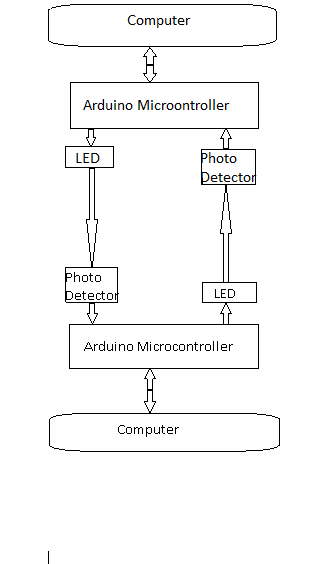
\includegraphics[width=9 cm , height= 12cm]{archi.png}
			\caption{Architecture}
		\end{figure}
	\end{center}
	
\textbf{user:}User can select which files to be sent and to which receiver.\\
\textbf{system: }System manages to establish connection between two devices.\\

 


\subsection{DATA DESIGN} 
The data stored is software data which is stored in file manager which is managed by OS. 

\subsubsection{Temporary data structure}
Queue data structure will be used for selecting files and sending in the order they arrive.
  
\subsubsection{Database description}
The data stored will be in Software data form which will vary according to the operating system.
\textbf{Module 1:} \\
	Software contains information like: \\
1.	User and device information\\
2.	File manager and information about filesystem.\\
3.	Selection of file from the filesystem. \\
\textbf{Module 2:}\\
	Hardware device contains the information like:\\
1.	Hardware structure\\
2.	Operational information related to sending or receiving file. \\
3.	Information about the operating software.\\ 




%------------DETAILED DESIGN DOCUMENT ends here----------




%%%%%
%%%%% Sem 2 Report starts here.
\newpage

\begin{minipage}{15cm}


\vspace{4 in}
 \begin{center} 
\begin{Huge}
CHAPTER 8

\vspace{0.5 in}

PROJECT IMPLEMENTATION
\end{Huge}

\end{center}
\end{minipage}

\newpage
\begin{center}
\section{PROJECT IMPLEMENTATION}
\end{center}
 {\setlength{\baselineskip}{1.0\baselineskip} 		
  \vspace{0.1in}
  
\subsection{INTRODUCTION}
 Nowadays,the transmission of data is becoming one of the most common factors among the computing devices. Various ways of data transmission have been enhanced such as WiFi, Bluetooth, etc. One of the most concerned issue about data transmission is data transmission security. A method needs to be developed which  will be provide both high speed data transmission as well as data transmission security. LiFi system is one of the emerging technology which is fast and easy to use.\\

\hspace{10 pt}Various methods are available today which provide data transmission feature among various devices. These can be wired or wireless protocols. However these protocols have been some limitations are filled up by LiFi data communication techniques. LiFi is advantages for achieving large data bandwidth which is the demand of the network using crowd.\\

\hspace{10 pt}Some of the network protocols are almost unusable in few situation. For example, WiFi cannot be used in establishing connection between two mountains. Another example can be communicating with submarines and the ships, which can also be achieved with the LiFi.
\\
\\
\subsection{TOOLS AND TECHNOLOGIES USED}
\\
\textbf{Java}\\
\hspace{10pt}Java is a general-purpose computer-programming language that is concurrent, class-based, object-oriented,[15] and specifically designed to have as few implementation dependencies as possible. One design goal of Java is portability, which means that programs written for the Java platform must run similarly on any combination of hardware and operating system with adequate runtime support. This is achieved by compiling the Java language code to an intermediate representation called Java bytecode, instead of directly to architecture-specific machine code. There are no. of Java compilers such as Eclipse, Javac, Intellij Idea, etc. In this project we used Intellij Idea.\\
\\
\textbf{IntelliJ IDEA}\\
\hspace{10 pt}IntelliJ IDEA is a Java integrated development environment (IDE) for developing computer software. It is developed by JetBrains (formerly known as IntelliJ). It is cross-platform and is primarily aimed at Java, Java EE and web development. An open-source version is available under the name IntelliJ IDEA Community Edition, and a proprietary version as IntelliJ IDEA Ultimate Edition, and is the most widely used for the Java development.\\
\\
\textbf{Arduino IDE}\\
The Arduino Integrated Development Environment - or Arduino Software (IDE) - contains a text editor for writing code, a message area, a text console, a toolbar with buttons for common functions and a series of menus. It connects to the Arduino and Genuino hardware to upload programs and communicate with them.\\
\hspace{10 pt}Programs written using Arduino Software (IDE) are called sketches. These sketches are written in the text editor and are saved with the file extension .ino. The editor has features for cutting/pasting and for searching/replacing text. The message area gives feedback while saving and exporting and also displays errors. The console displays text output by the Arduino Software (IDE), including complete error messages and other information. The bottom righthand corner of the window displays the configured board and serial port. The toolbar buttons allow you to verify and upload programs, create, open, and save sketches, and open the serial monitor.\\
\\
\subsection{VERIFICATION AND VALIDATION FOR ACCEPTANCE}
\begin{itemize}
\item Software verification
It is the process of evaluating a system or component to determine whether the product of given development phase satisfy the condition imposed at the start of the phase.
\begin{enumerate}
\item It is a static process
\item It does not involve any code and is human based checking.
\item It uses methods like inspections,walk through,desk checking etc.
\item It can catch errors that validations cannot.
\end{enumerate}
\item Software validation
\end{itemize}
It is the process of evaluating a system or component during or at the end of the development process to determine to determine whether it specifies the specified requirements. It involves executing the actual software.it is a computer based testing process.
\begin{enumerate}
\item It is a dynamic process.
\item It involves executing of code as well as human based execution of program.
\item It uses methods like Black box and white box testing.
\item It can catch errors that verification cannot catch. Note that verification and validation
\end{enumerate}
(V and V') are complementary to each other.
V and V' is a technical discipline of system engineering. Software V and V' is a system engineering process employing a rigorous methodology for evaluating the correctness and quality of software product through the software life cycle.

  
%------------DETAILED DESIGN DOCUMENT ends here----------

%%%%%
\newpage
\newpage
\begin{minipage}{15cm}


\vspace{4 in}
 \begin{center} 
\begin{Huge}
CHAPTER 9

\vspace{0.5 in}
SOFTWARE TESTING

\end{Huge}

\end{center}
\end{minipage}

\newpage
\begin{center}
\section{SOFTWARE TESTING}
\end{center}
\subsection{TYPE OF TESTING USED}
\begin{itemize}
\item\textbf{Unit Testing:}\\
It is the testing of individual software units of the application .it is done after the completion of an individual unit before integration. Unit testing involves the design of test cases that validate that the internal program logic is functioning properly, and that program inputs produce valid outputs. All decision branches and internal code flow should be validated. This is a structural testing, that relies on knowledge of its construction and is invasive.
Unit tests perform basic tests at component level and test a specific business process, application, and/or system configuration. Unit tests ensure that each unique path of a business process performs accurately to the documented specifications and contains clearly defined inputs and expected results.\\
\textbf{Benefits:}\\
The goal of unit testing is to isolate each part of the program and show that the individual parts are correct. A unit test provides a strict, written contract that the piece of code must satisfy. As a result, it affords several benefits.
\item\textbf{Integration Testing:}\\
Integration tests are designed to test integrated software components to determine if they actually run as one program.  Testing is event driven and is more concerned with the basic outcome of screens or fields. Integration tests demonstrate that although the components were individually satisfaction, as shown by successfully unit testing, the combination of components is correct and consistent. Integration testing is specifically aimed at   exposing the problems that arise from the combination of components.\\
\textbf{Purpose:}\\
The purpose of integration testing is to verify functional, performance, and reliability requirements placed on major design items. These "design items", i.e., assemblages (or groups of units), are exercised through their interfaces using black box testing, success and error cases being simulated via appropriate parameter and data inputs. Simulated usage of shared data areas and inter-process communication is tested and individual subsystems are exercised through their input interface. Test cases are constructed to test whether all the components within assemblages interact correctly, for example across procedure calls or process activations, and this is done after testing individual modules, i.e., unit testing. The overall idea is a "building block" approach, in which verified assemblages are added to a verified base which is then used to support the integration testing of further assemblages.
Software Integration Testing is performed according to the Software Development Life Cycle (SDLC) after module and functional tests. The cross-dependencies for software integration testing are: schedule for integration testing, strategy and selection of the tools used for integration, define the cyclomatical complexity of the software and software architecture, reusability of modules and life-cycle / versioning management.\\ Some different types of integration testing are big bang, top-down, and bottom-up, mixed (sandwich) and risky - hardest. Other Integration Patternsare: Collaboration Integration, Backbone Integration, Layer Integration, Client/Server Integration, Distributed Services Integration and High-frequency Integration.

\item\textbf{System Testing:}\\
System Testing is the testing of a complete and fully integrated software product.Usually software is only one element of a larger computer based system. Ultimately, software is interfaced with other software/hardware systems.System Testing is actually a series of different tests whose sole purpose is to exercise the full computer based system.\\ \\
\textbf{Two Category of Software Testing: }
\item Black Box Testing
\item White Box Testing

System test falls under the black box testing category of software testing.\\White box testing is the testing of the internal workings or code of a software application. In contrast, black box or System Testing is the opposite. System test involves the external workings of the software from the user's perspective.
\end{itemize}
\\

\subsection{TEST CASES AND TEST RESULTS}
\\
Write test Cases ans Test Results
%%%%%%%%%%%%%%%%%%Chapter 9 Ends%%%%%%%%%%%
\newpage
\begin{minipage}{15cm}


\vspace{4 in}
 \begin{center} 
\begin{Huge}
CHAPTER 10

\vspace{0.5 in}

RESULTS
\end{Huge}

\end{center}
\end{minipage}

\newpage
\begin{center}
\section{RESULTS}
\end{center}

\subsection{SCREEN SHOTS}

\subsection{OUTPUTS}



%%%%%%%%%%%%%%Chapter 10 ends here.%%%%%%%%%%%%%%%%
\newpage
\begin{minipage}{15cm}


\vspace{4 in}
 \begin{center} 
\begin{Huge}
CHAPTER 11

\vspace{0.5 in}

DEPLOYMENT AND MAINTENANCE
\end{Huge}

\end{center}
\end{minipage}

\newpage
\begin{center}
\section{DEPLOYMENT AND MAINTENANCE}
\end{center}

\subsection{INSTALLATION AND UN-INSTALLATION}

\subsection{USER HELP}



DEPLOYMENT AND MAINTENANCE
%%%%%%%%%%%%%%%%%Chapter 11 Ends here.%%%%%%%%%%%%%%%




\newpage
\begin{minipage}{15cm}


\vspace{4 in}
 \begin{center} 
\begin{Huge}
CHAPTER 12


\vspace{0.5 in}

SUMMARY AND CONCLUSION
\end{Huge}

\end{center}
\end{minipage}

\newpage
% \pagenumbering{arabic}
\begin{center}
\section{SUMMARY AND CONCLUSION}
\end{center}
 {\setlength{\baselineskip}{1.0\baselineskip} 		
  \vspace{0.1in}	
 
%---------------SUMMARY AND CONCLUSION ends here-----------------



\hspace{10 pt} 
After running few tests and inspecting the results we have concluded that the proposed system is capable of transmitting data with satisfactory speed. All the hardware devices are found to be working properly as expected. It has been concluded that the LiFi system proposed will be useful for most of the people and will be able to solve various issue related to security. System is also capable of allowing to make any change if needed. 
\\






%-------------------------References---------------------------
\begin{appendices}
\newpage
\begin{minipage}{18cm}


\vspace{4 in}
 \begin{center} 
\begin{Huge}

ANNEXURE A

\vspace{0.5 in}
REFERENCES
\end{Huge}

\end{center}
\end{minipage}
\newpage
\newpage
\begin{center}
\section{REFERENCES }
\end{center}


\hspace{[1]} Zashi P. Chaudhari, Satish R. Devane, "High sensitivity universal LiFi receiver for enhanced data communication", IEEE, 2016.\\
\hspace{[2]} Monica Leba, Simona Riurean, Andreea Lonica, "LiFi The path to a New Way of Communication", IEEE, 2017. \\
\hspace{[3]} Authors:R. Mahendran, "Integrated LiFi (Light Fidelity) for smart communication through illumi-
nation",IEEE,  2016.\\
\hspace{[4]} Harald Hass, "LiFi: Conceptions, misconceptions and opportunities",IEEE,  2016.\\
\hspace{[5]} Pradeep Kumar, "Future internet and Internet of things", IEEE, 2017.\\
\hspace{[6]} Kun Chen Hu, "Prototyping and measurements for a LiFi system", IEEE, 2016.\\
\hspace{[7]} Dahmani Mohammed, "Digital data transmission via visible light communication(VLC): Applica-
tion vehicle to vehicle communication", IEEE, 2016.\\
\hspace{[8]} Wasiu O. Popoola, "Impact of VLC on Light Immission Quality of White LEDs", IEEE, 2016.\\
\hspace{[9]} Wasiu O.Popoola, "On visible light communication and quality of light emitted from illumi-
nation LEDs", IEEE, 2016.\\


% \end{thebibliography}



%----------------------------------------Axxenure Begins here------------------



\newpage
\begin{minipage}{15cm}


\vspace{4 in}
 \begin{center} 
\begin{Huge}

ANNEXURE B

\vspace{0.5 in}
\setlength{\baselineskip}{1\baselineskip}
{ LABORATORY ASSIGNMENTS ON \\
PROJECT ANALYSIS OF ALGORITHMIC DESIGN \\}
\end{Huge}

\end{center}
\end{minipage}


\newpage
\section{Laboratory assignments on Project Analysis of Algorithmic Design}


{\large \underline{\textbf{Aim}:}}  {To develop the problem under consideration and justify 
feasibility using concepts of knowledge canvas and IDEA Matrix}. 

\textunderscore \textunderscore \textunderscore \textunderscore 
\textunderscore \textunderscore \textunderscore \textunderscore 
\textunderscore \textunderscore \textunderscore \textunderscore 
\textunderscore \textunderscore \textunderscore \textunderscore 
\textunderscore \textunderscore \textunderscore \textunderscore 
\textunderscore \textunderscore \textunderscore \textunderscore 
\textunderscore \textunderscore \textunderscore \textunderscore 
\textunderscore \textunderscore \textunderscore \textunderscore 
\textunderscore \textunderscore \textunderscore \textunderscore 
\textunderscore \textunderscore \textunderscore \textunderscore 
\textunderscore \textunderscore \textunderscore \textunderscore 
\textunderscore \textunderscore \textunderscore \textunderscore 
\textunderscore \textunderscore \textunderscore \textunderscore 
\textunderscore \textunderscore \textunderscore \textunderscore 
\textunderscore \textunderscore \textunderscore \textunderscore 
\textunderscore \textunderscore \textunderscore \textunderscore 
\textunderscore \textunderscore \textunderscore \textunderscore 
\textunderscore \textunderscore \textunderscore \textunderscore 
\textunderscore \textunderscore \textunderscore 
\textunderscore \textunderscore \textunderscore \textunderscore 
\textunderscore \textunderscore \textunderscore
\\



{ \large{ \underline{ \textbf{IDEA MATRIX: }}}

\begin{center}
 \begin{tabular}{|p{100pt}|p{100pt} | p{100pt} | p{100pt} |} 

 \hline

 \textbf{ I} & \textbf{D} & \textbf{E} & \textbf{A} \\ 
 \hline
 \underline {\textbf{INCREASE: }} \par Speed of the Data transmission and  provide data transmission security to the user.
 . \par &
 
  \underline {\textbf{DRIVE: }} \par Interaction between Developer and File managing Environment \par  &
  
  \underline {\textbf{EDUCATE:}} \par The API can be used to perform faster data transmission and provide security to the users.
\par & 
  
\underline {\textbf{ACCELERATE:}} \par Transmission speed and better resource utilisation. \par  
  \\
 \hline

 

 \underline {\textbf{IMPROVE: }} \par 
Speed of transmission and security. \par &
 
  \underline {\textbf{DELIVER:: }} \par Better performance . \par  &
  
  \underline {\textbf{EVALUATE:}} \par Maximum data transmission in minimum time. \par & 
  
\underline {\textbf{ASSOCIATE:}} \par Multiple users or group of people.

\par  
  \\
 \hline



 
 
\underline{  \textbf{IGNORE:} } \par Interference of outer lights. \par &
 
\underline{  \textbf{DECREASE: :} } \parTime required for data transmission.
\par &
  
 
\underline{  \textbf{ELIMINATE:} } \par Limitation of one
 way communication 
.\par &
 
\underline{  \textbf{AVOID:} } \par Radiation due to 
data transmission

 \par
 \\
 
 \hline
\end{tabular}
\end{center}

\vspace{50pt}
\newpage

%%%%%%%%%%%%%%%%%%%%%%%%%%%%%%%%%%%newpage%%%%%%%%%%%%%%%%%%%%%%%%%%%%%%%%%

{\large \underline {\textbf{I }}}
\\
\begin{center}
 \begin{tabular}{|p{80pt}|p{140pt}  | p{140pt} |} 
 
 
 \hline


  \underline {\textbf{INCREASE: }} &
  \parSpeed of the Data and 
  provide data transmission security.

 &
\par User gets the  
better transmission 
speed, security, quality
and better interface
 with System.
\\
\hline 


\underline {\textbf{IMPROVE: }} &
  \par Speed of transmission and security.&
\par	Better Performance and increased speed. 
\\
\hline 


\underline {\textbf{IGNORE: }} &
  \parHardware Interference of outer lights.  &
\par	Doesn’t interface with external lights.

\\
\hline 


\end{tabular}
\end{center}

\vspace{45 pt}

{\large \underline {\textbf{D }}}
\\
\begin{center}
 \begin{tabular}{|p{80pt}|p{140pt}  | p{140pt} |} 
 
 
 \hline


  \underline {\textbf{DRIVE:  }} &
  \par Interaction between developer and File manager.
 &
\par 	Developer will use Java to interact and build simple API.
\\
\hline 


\underline {\textbf{DELIVER: }} &
  \par Better performance.  &
\par	Faster data transmission and desired output.
\\
\hline 


\underline {\textbf{DECREASE: }} &
  \par Time required for data transmission. &
\parReduce human efforts of manual data transmission .
\\
\hline 


\end{tabular}
\end{center}

\newpage

%%%%%%%%%%%%%%%%%%%%%%%%%%%%%%%%%%%newpage%%%%%%%%%%%%%%%%%%%%%%%%%%%%%%%%%

{\large \underline {\textbf{E }}}
\\
\begin{center}
  \begin{tabular}{|p{80pt}|p{140pt}  | p{140pt} |} 
 
 
 \hline


  \underline {\textbf{EDUCATE: }} &
  \par The API can be used to perform faster data transmission and provide security to user.
 &
\par We can use this technology to improve day-to-day human life
\\
\hline 


\underline {\textbf{EVALUATE: }} &
  \par Maximum data transmission in minimum time.
   &
\par	Better transmission rate with user data security.  
\\
\hline 


\underline {\textbf{ELIMINATE: }} &
  \par Limitation of one way Communication.
    &
\par	Provides two way communication and eliminates slow data transfer.


\\
\hline 


\end{tabular}
\end{center}

\vspace{25 pt}


{\large \underline {\textbf{A }}}
\\
\begin{center}
 \begin{tabular}{|p{80pt}|p{140pt}  | p{140pt} |}
 
 
 \hline


  \underline {\textbf{{\small ACCELERATE:} }} &
  \par Transmission speed and better resource utilization.
  &
\par 	The system aims to accelerate the transmission speed and focuses on resource utilisation through Java API. 
\\
\hline 





\underline {\textbf{{\small ASSOCIATE:} }} &
  \par  Multiple users or Group of people.
 &
\par	 Multiple users can use it. 
\\
\hline
\underline {\textbf{{\small AVOID:}  }} &
  \par Radiation due to data transmission

   &
\par	Avoids radiation effects which was caused by traditional wireless .



\\
\hline 
 


\end{tabular}
\end{center}
}

%--------------------end of IDEA matrix----------------

\newpage
\textbf{
{\large Feasibility assessment using NP-Hard, NP-Complete:}}

\vspace{30pt}
\textbf{NP-Complete problems} are the problems that can be solved by using NP-Complete algorithms. NP-Complete algorithms (Non-Deterministic algorithms) are the algorithms in which every operation may not have unique result, rather there can be specified set of possibilities for every operation.
NP-Complete means that no particular rule is followed to make a guess. Therefore the outcome or result is not predictable. \\
\par
NP-complete problems are in NP, the set of all decision problems whose solutions can be verified in polynomial time; NP may be equivalently defined as the set of decision problems that can be solved in polynomial time on a non-deterministic Turing machine. A problem p in NP is NP-complete if every other problem in NP can be transformed (or reduced) into p in polynomial time

\vspace{20pt}

\textbf{NP-Hard problems:} These problems are the problems in which the solutions are not found using multiple algorithms that is problems that are not solvable are NP-Hard problems. 
\\
\par
NP-hardness (non-deterministic polynomial-time hard), in computational complexity theory, is a class of problems that are, informally, "at least as hard as the hardest problems in NP". More precisely, a problem H is NP-hard when every problem L in NP can be reduced in polynomial time to H, that is given a solution for L we can verify it is a solution for H in polynomial time.
\\
As a consequence, finding a polynomial algorithm to solve any NP-hard problem would give polynomial algorithms for all the problems in NP, which is unlikely as many of them are considered hard.\\
%---------------------------------------------------------------------------------------

\newpage
\begin{minipage}{18cm}
\vspace{4 in}
 \begin{center} 
\begin{Huge}

ANNEXURE C

\vspace{0.5 in}
\setlength{\baselineskip}{1\baselineskip}
LABORATORY ASSIGNMENTS ON \\
PROJECT QUALITY AND RELIABILITY \\
TESTING OF PROJECT DESIGN \\
\end{Huge}

\end{center}
\end{minipage}

\newpage

\section{Laboratory assignments on Quality and Reliability Testing of Project Design}


 Use of divide and conquer strategies to exploit distributed/parallel/concurrent processing of the above to identify object, morphisms, overloading in functions (if any), and functional relations and any other dependencies (as per requirements).
            Our system work as a distribute manner. It means that one module is dependant on the another module. The output of previous module is required as a input to the next module. So that before executing previous  module we cannot execute the next module.
 Use of above to draw functional dependency graphs and relevant Software modeling methods, techniques including UML diagrams or other necessities using appropriate tools.
 \vspace{20 pt}
 
\textbf{ Software Testing:-}\\
Software testing is the process of evaluation a software item to detect differences between given input and expected output. Also to access the feature of a software item. Testing assesses the quality of the product. Software testing is a process that should be done during the development process. In other words software testing is a verification and validation process.\\
 \vspace{20 pt}
\textbf{Verification:}\\
Verification is the process to make sure the product satisfies the conditions imposed at the start of the development phase. In other words, to make sure the product behaves the way we want it to.\\
 \vspace{20 pt}
\textbf{Validation:}\\
Validation is the process to make sure the product satisfies the specified requirements at the end of the development phase. In other words, to make sure the product is built as per customer requirements.\\


%-------------------------------------------------------------------------------------------


\newpage
\begin{minipage}{15cm}


\vspace{4 in}
 \begin{center} 
\begin{Huge}

ANNEXURE D

\vspace{0.5 in}
PROJECT PLANNER
\end{Huge}

\end{center}
\end{minipage}




\newpage
\section{Project Planner}
\label{app:plan}
Project planning emphasizes on following aspects: \\
\textbf{{Work Breakdown:}} \\
\hspace{0.5 in} Load the Work Breakdown Structure data into the planning and scheduling repositories. As the Work Breakdown Structure content is derived, progressively load the data into the planning and scheduling repositories. Generate reports, review the content and progressively update the data. This process continues on an iterative basis.\\
 Requirement Analysis and study part of the project was as follows:
\begin{itemize}
\item Understanding the problem definition;
\item Understanding the current scenario in Market;
\item Gathering information about required Software;
\item Gathering information about required Software Resources;
\item Preparing preliminary design of overall work flow of project;
\item Deciding the modules required for overall execution.
\end{itemize}

\begin{center}
	  \begin{figure}[h]
			\centering
			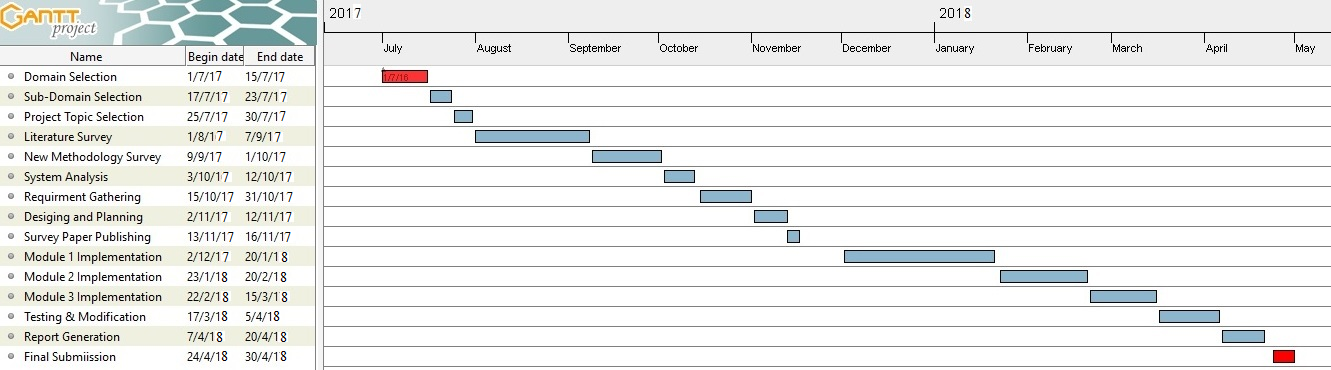
\includegraphics[width=17 cm , height= 8 cm]{TC.png}
		
		\end{figure}
		Fig : Timeline Chart
	\end{center}
%---------------------------------------------------------------------------------------------
\newpage
\begin{minipage}{18cm}
\vspace{4 in}
 \begin{center} 
\begin{Huge}

ANNEXURE E

\vspace{0.5 in}
\setlength{\baselineskip}{1\baselineskip}
{
REVIEWERS COMMENTS OF PAPER \\ 
SUBMITTED\\
}
\end{Huge}

\end{center}
\end{minipage}

\newpage
\section{Reviewers Comments of Paper submitted}
\begin{enumerate}
\item \textbf{Paper Title:}  `` High Speed Data Communication using LiFi providing Security";
\item \textbf{Name of the conference/Journal where paper submitted :} \\ IJCA (``International Journal of Computer Applications")	, Vol. 5, Issue Jan 2018; \\
\item \textbf{Paper accepted/rejected:  } ``Under Scrutiny";
\\
\item \textbf{Review comments by reviewer:}\\
1. Subject Content is good \\
2. Technical Content is good.\\
3. Contribution to the field is satisfactory. \\
4. Depth of Research is good.\\
5. Presentation is satisfactory.\\
\item \textbf{Corrective actions:} ``Font size changes ";
\end{enumerate}
%-------------------------------------------------------------------------------
\newpage
\begin{minipage}{15cm}
\vspace{4 in}
 \begin{center} 
\begin{Huge}

ANNEXURE F

\vspace{0.5 in}
PLAGIARISM REPORT
\end{Huge}

\end{center}
\end{minipage}

\newpage
\section{Plagiarism Report}
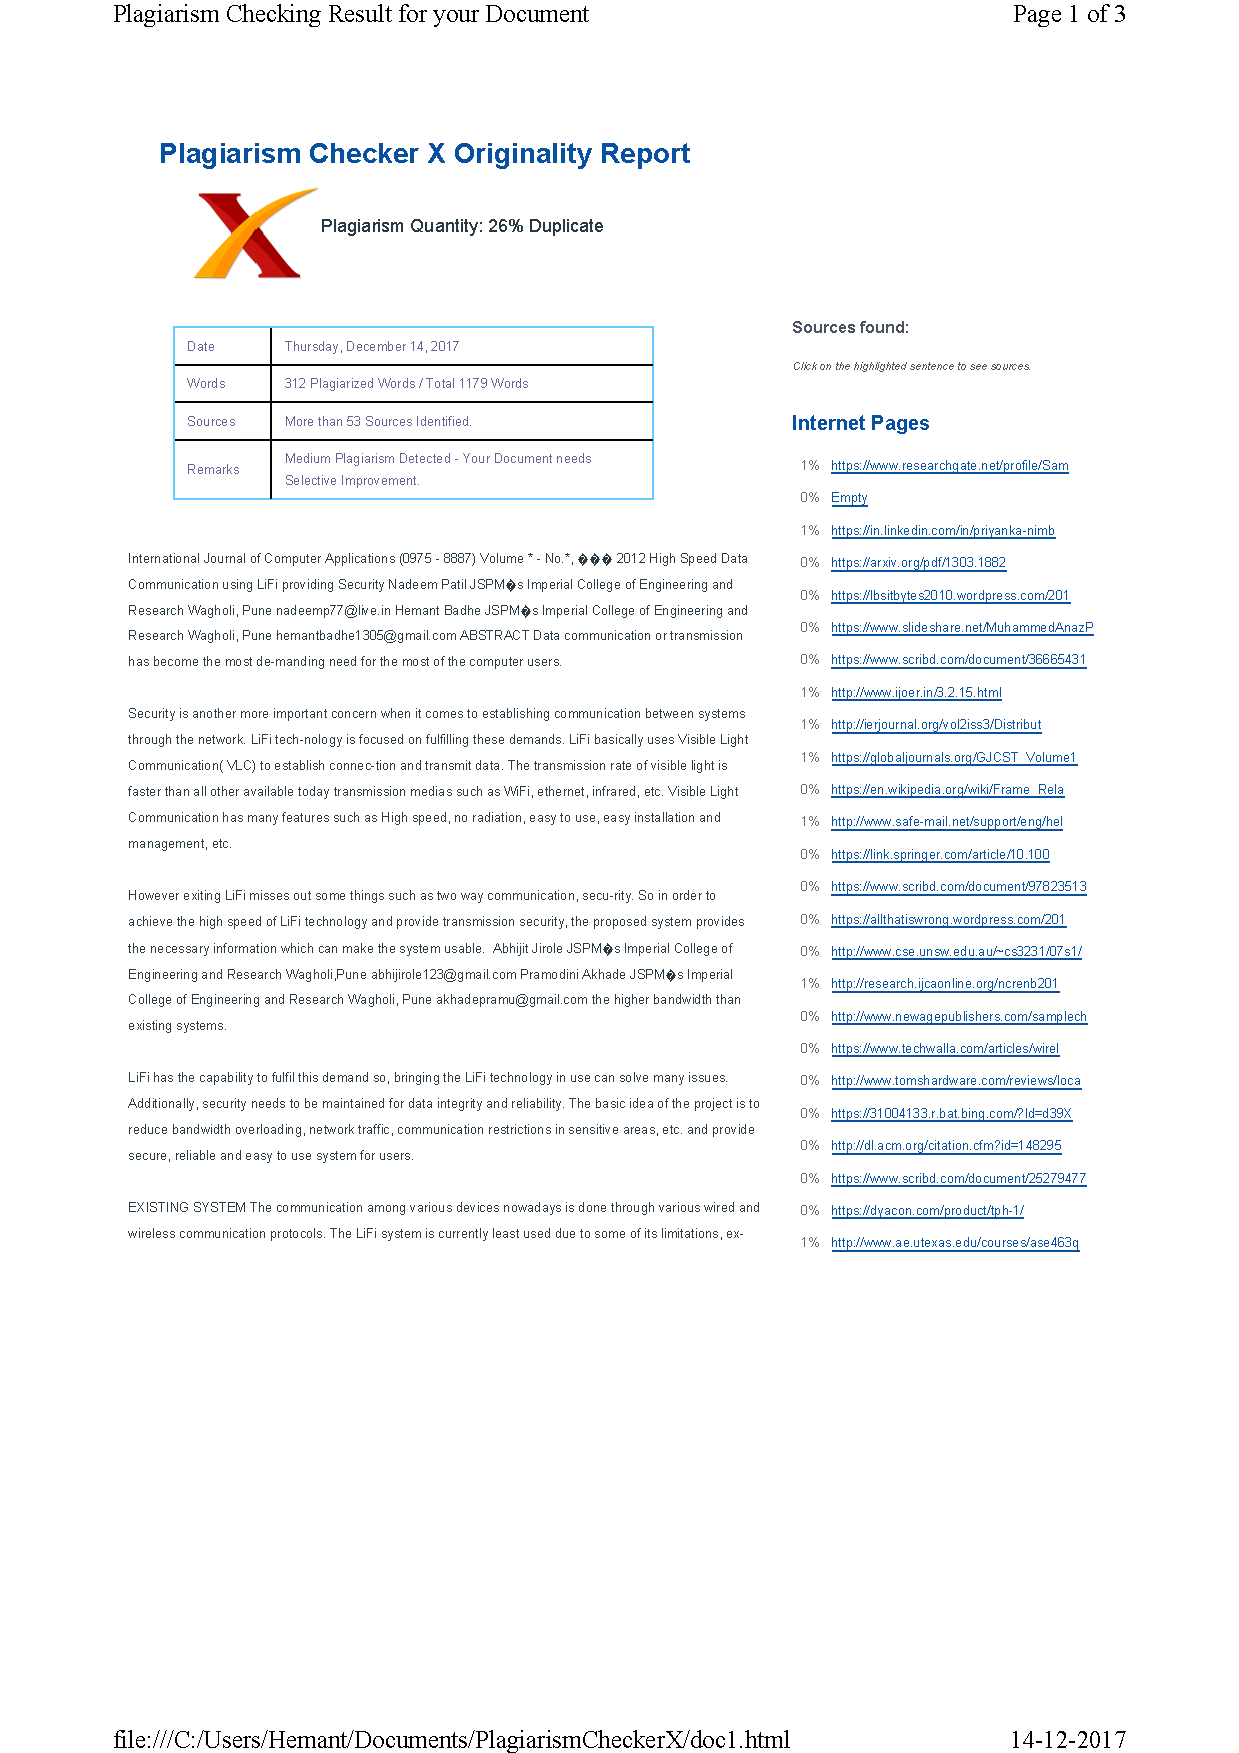
\includepdf[pages=-]{plag_report.pdf}
%%%%%%%%%%%%%%%%%%%%%%%%%%%%%%%%%%%%%%%%%%%%%%%%%%%%%%%%%%%%%%%%

\newpage
\begin{minipage}{15cm}
\vspace{4 in}
 \begin{center} 
\begin{Huge}

ANNEXURE G

\vspace{0.5 in}
INFORMATION OF PROJECT GROUP
MEMBERS
\end{Huge}
\end{center}
\end{minipage}

\newpage
\begin{enumerate}
\item Name : Nadeem A. Patil \hspace{90 mm}\includegraphics[width=60pt]{photo.jpg}
\item Date of Birth : 30th Jan 1997
\item Gender : Male
\item Permanent Address : Narmada Park, Solapur.
\item E-Mail : nadeempatil@gmail.com
\item Mobile/Contact No. : 9762973167
\item Placement Details : Placed.
\item Paper Published : 
\\
\newpage
\begin{enumerate}
\item Name : Abhijit D. Jirole \hspace{90 mm}\includegraphics[width=60pt]{photo.jpg}
\item Date of Birth : 25th May 1997
\item Gender : Male
\item Permanent Address : Malighogargaon, Solapur.
\item E-Mail : abhijirole123@gmail.com
\item Mobile/Contact No. : 7030728340
\item Placement Details : Not Placed.
\item Paper Published : 
\\
\newpage
\begin{enumerate}
\item Name : Hemant B. Badhe \hspace{90 mm}\includegraphics[width=60pt]{photo.jpg}
\item Date of Birth : 13th May 1997
\item Gender : Male
\item Permanent Address : Gondegaon, Shrirampur
\item E-Mail : hemantbbadhe@gmail.com
\item Mobile/Contact No. : 9730462723
\item Placement Details : Not Placed.
\item Paper Published : 
\\
\newpage
\begin{enumerate}
\item Name : Pramodini B. Akhade \hspace{90 mm}\includegraphics[width=60pt]{photo.jpg}
\item Date of Birth : 14th Sep 1996
\item Gender : Female
\item Permanent Address : Maka, Newasa.
\item E-Mail : pramuakhade@gmail.com
\item Mobile/Contact No. : 9657991524
\item Placement Details : Not Placed.
\item Paper Published : 
\end{enumerate}
\end{appendices}
\end{document}

